\section{Methods}
\label{section:methods}
Many components are necessary to successfully train an agent using reinforcement learning. Reinforcement learning is notoriously tricky to train, and so are spiking neural networks. Therefore, the choice of agent architectures, loss functions, neuron models etc. are of utmost importance. First the background of the reinforcement algorithm being used will be explained. Then, the network responsible for interacting with the environment is presented. Finally, the training of the algorithm is elaborated upon.

\subsection{A2C Reinforcement Learning}
In 2016, DeepMind introduced the Asynchronous Advantage Actor-Critic (A3C) algorithm in their paper \textit{Asynchronous Methods for Deep Reinforcement Learning} \cite{A3C}. It is built on using multiple workers who explore the environment in parallel independently and updating a global network with their experiences, asynchronously. Before a worker interacts with its environment, it updates its internal model with the global model. Compared to the popular DQN algorithm, this network did not need experience replay, trying to reduce variance and bias by using the experience from multiple workers, and thus updates the underlying model more frequently with fresh experiences. While the A3C algorithm performed well on many tasks, it was unsure whether the asynchrony, which adds complexity, actually affected the performance positively. Next to the added complexity, A3C does not take full advantage of the possibility to perform computations on large batch sizes of the GPU. Therefore, the synchronous version of A3C has been introduced, named Advantage Actor-Critic (A2C). As the ability to perform online distributed training with these algorithms shows promising avenues for fine-tuning after deployment, we decided to pursue experimentation using these algorithms rather than the DQN based algorithms, which already showed promising results. When finetuning on device, every sample is costly to obtain. Having to wait until sufficient experience has been gathered to start training, is therefore undesirable.
\\
\subsection{CartPole task}
The task to be solved in this article is the CartPole task. This task has been widely used to develop new reinforcement learning algorithms due to its simple implementation, yet challenging solution. The task consists of balancing a pole on a cart as long as possible, receiving $+1$ reward for every timestep where the pole is balanced. The actor can apply either a force to the left or to the right on the cart, while observing the position and velocity of the cart and angle and angular velocity of the pole. For all models, the environment is ran at a frequency of 20Hz. 
\subsection{Architecture and Neuron Model}
Where the conventional reinforcement learning methods use actor-critic models based on a deep neural network using artificial neurons, the aim of this article is to demonstrate the use of spiking neural networks. Spiking neural networks use biologically inspired neuron models that simulate the behavior of neurons in the brain. In the past, many different neuron types have been proposed, with each their specific use cases. Complex neuron models are often utilized for neuroscience research, while simpler models have shown useful in machine learning research. \\

To compare ANN to SNN, two models (an ANN and an SNN) with the same architecture were used. The only difference between the models is the spiking neurons in the SNN, replacing the regular activation functions. This architecture is kept small to avoid long training times, which is an issue for SNN. The input layer consists of 4 continuous neurons, there is one hidden layer, with 246 neurons, and finally, two output heads represent the actor and critic output respectively. Next to this shallow network, experiments were carried out with a slightly deeper network with a similar number of neurons. This second architecture replaces the single hidden layer with 246 neurons, with two hidden layers, each having 128 neurons.\\

The activation function used for the ANN is the ReLU function. In the SNN experiments were conducted with two different neuron types for the hidden layer, and a non-spiking equivalent of each respective neuron is used for the output layer. Firstly, the leaky integrate fire (LIF) is used. The LIF neuron is a first-order neuron where the input current, $I_{in}$ directly charges the membrane potential, $U$. This potential energy leaks over time at a rate $\beta$, the leakage parameter. When this potential exceeds a threshold, $U_{thr}$, the neuron spikes and the membrane potential is reset, by subtracting the threshold value. The charging and resetting of the membrane potential can be modeled using the following equation:
\begin{equation}
    U[t+1] = \beta U[t] + I_{in}[t+1] - R\cdot U_{thr}
\end{equation}
Where $R$ is 1 whenever the membrane potential exceeds the threshold and 0 otherwise.
The spiking behavior can be modeled as:
\begin{equation}
    s = \begin{cases}
           1,& \text{if } U[t+1] > thr\\
    0,              & \text{otherwise} 
    \end{cases}
\end{equation}
Alternatively, a second order model, namely a synaptic neuron model was investigated as well. In second order models, the synaptic current is charged by the input current, which subsequently charges the membrane potential, after which similar behavior as the LIF can be observed. Concretely, the following equations model these dynamics.
\begin{align}
    I_{syn}[t+1] &= \alpha I_{syn}[t] + I_{in}[t+1]\\
    U[t+1] &= \beta U[t] + I_{syn}[t+1] - R U_{thr}
\end{align}
The spiking behavior for this neuron is the same as the LIF neuron described above. However, after initial experiments, it was found that this neuron model showed very slow convergence. After analyzing the impulse response of this neuron type, it is found that it is significantly delayed compared to the first order model, which might be a cause for the slow training.\\

\subsection{Encoding and Decoding}
To deploy spiking based models, we have to translate the continuous domain to the discrete spiking domain and back to continuous domain at the output. The way the bridging of domains is carried out has significant effects on training speed and final model performance. Several successful methods have been proposed in the past, ranging from rate coded, latency coded to population coded methods. For robotic applications, learned coding has shown effective and easy to implement\cite{stroobants_neuromorphic_2022}. The continuous inputs are connected to a first layer of spiking neurons with a simple linear layer that encodes the continuous input to input current, which is fed into the first spiking layer. The output is directly read from the membrane potential from the last layer, which is programmed to never spike. While this method can learn complicated encoding and decoding mechanisms, it is not necessarily the most computationally efficient method. Depending on the layer sizes, large linear layers might be required, for which the number of multiply-accumulates equals the product of the matrix dimensions.

\subsection{Training Spiking Neural Networks}
Training spiking neural networks have shown to carry several unique challenges. Firstly, due to the discrete spiking nature of the neurons, one can not compute the derivative of this activation to compute the gradient of the weights running through the network. Therefore, several different training methods have been proposed. To be able to apply a reinforcement learning algorithm without significant changes to train an SNN, we would like to have a training method based on backpropagation. To find the gradient of the non-differentiable spikes, a surrogate gradient is applied during the backward pass\cite{neftci2019surrogate}. When training using surrogate gradients, a continuous, differentiable function is used to mimic the spiking behavior. During the forward pass, the discrete spiking function is used, but during the backward pass, the derivative surrogate gradient represents the gradient of the signal through the network. The derivative of this surrogate function is a real non-zero value at the time of spiking. Its trace reduces to zero as time moves away from the spike time, seen on \autoref{fig:surrogate}. The surrogate function used is the fast sigmoid function with a slope of 25. Increasing the slope leads to shorter traces in time. \\
\begin{figure}[h]
    \centering
    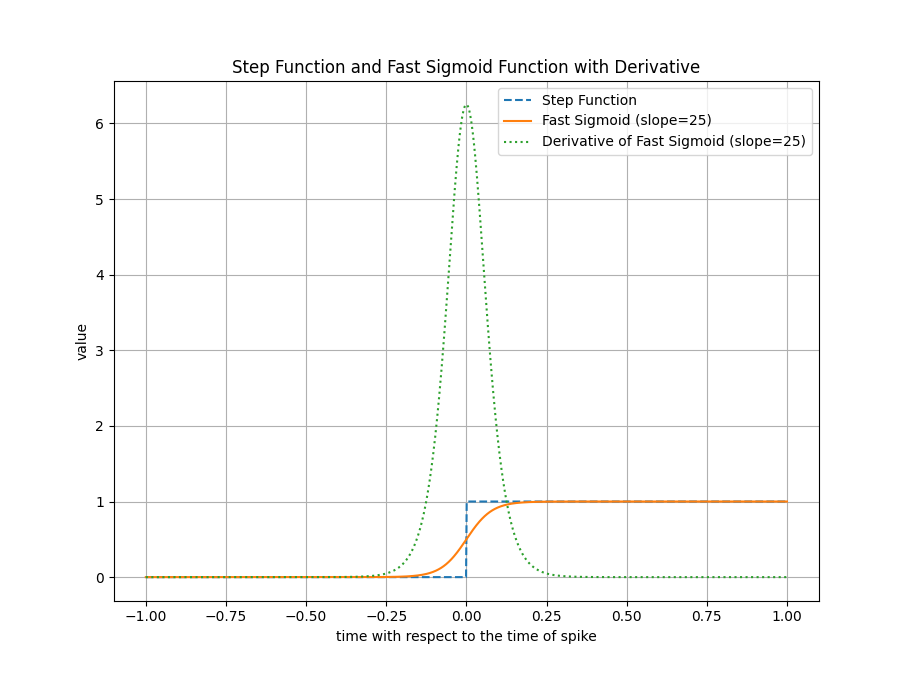
\includegraphics[width=0.45\textwidth]{Figures/surrogate.png}
    \caption{The step function, surrogate function and its gradient.}
    \label{fig:surrogate}
\end{figure}
Next to the above-mentioned challenges, the choice of loss function effects the training process significantly. For policy gradient methods, generalized advantage can improve sample efficiency and increase stability during training~\cite{schulman_high-dimensional_2018}. This loss was applied to the membrane potentials of the output neurons.

\subsection{Pruning the Spiking Neural Network}
To explore opportunities of using the trained agents on resource-constrained embedded devices, pruning and quantization are widely used to reduce the footprint and computational effort of networks. While in ANN, spatial pruning is extensively exploited, in SNN the opportunity rises to take a temporal pruning approach, with minimal performance decay. Due to undesired effects during training using RL, the trained agent often has dead or saturated spiking neurons. Dead neurons are the ones that never spike, while saturated spiking neurons spike at every timestep. This opens the opportunity to prune the network without losing any performance. Dead neurons, and the connecting weights, can be removed. Saturated spiking neurons, on the other hand, can be removed by removing the weights connecting it to the previous layer, and adding the weights connecting to the next layer as bias of the next neuron layer.
